\question 下列有关设备独立性的说法中正确的是
\par\fourch{设备独立性是指I/O设备具有独立执行I/O功能的一种特性}{\textcolor{red}{设备独立性是指用户程序独立于具体物理设备的一种特性}}{设备独立性是指能够实现设备共享的一种特性}{设备独立性是指设备驱动程序独立于具体物理设备的一种特性}
\begin{solution}设备独立性是指用户程序独立于具体物理设备的一种特性。其他选项都不是设备独立性的描述。D选项错在设备驱动程序是不可能独立于具体物理设备的,因为驱动程序就是为具体物理设备而专门定制的。
\end{solution}
\question 用户程序发出磁盘I/O请求后,系统的正确处理流程是( )
\par\fourch{用户程序→系统调用处理程序→中断处理程序→设备驱动程序}{\textcolor{red}{用户程序→系统调用处理程序→设备驱动程序→中断处理程序}}{用户程序→设备驱动程序→系统调用处理程序→中断处理程序}{用户程序→设备驱动程序→中断处理程序→系统调用处理程序}
\begin{solution}首先用户程序(目态)是不能直接调用设备驱动程序的,因为有关对I/O设备使用的指令是特权指令,只能通过系统调用,把进程的状态从用户态变为核心态,故C、D选项错误。
I/O软件一般从上到下分为图19-1所示的4个层次:用户层、设备独立性软件层、设备驱动程序及中断处理程序。设备独立性软件也就是系统调用的处理程序。因此正确处理流程为B。
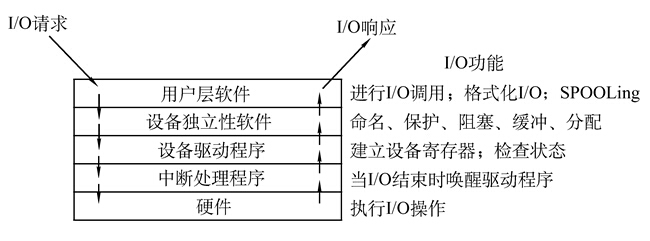
\includegraphics[width=6.77083in,height=2.51042in]{computerassets/6dbc4c72f9dd72ff8544000ba5bc7d05.jpeg}
【总结】
图中的箭头表示I/O控制流。当用户程序试图从文件中读一个数据块时,需要通过操作系统来执行此操作。设备独立性软件通过系统调用启动设备驱动程序向硬件发出相应的请求,用户进程随即阻塞直到数据块被读出。当磁盘操作完成时,硬件产生一个中断,并转入中断处理程序。中断处理程序检查中断的原因,并从设备获取所需的信息,然后唤醒睡眠的进程以结束此次I/O请求,使用户进程继续执行。
\end{solution}
